\documentclass[t]{beamer}
\usepackage{listings}
\usepackage{minted}

\usetheme{default}
\usebackgroundtemplate{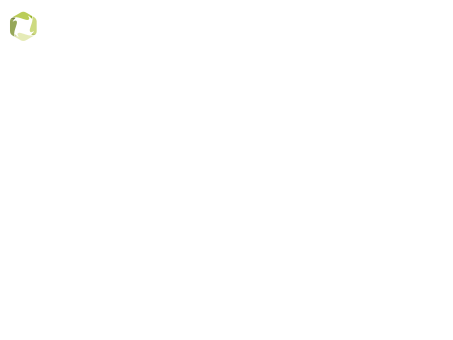
\includegraphics[width=\paperwidth]
                                       {../cpeb_bkground_topleftlogo.pdf}}

\setbeamertemplate{frametitle}{
  \centering\vspace{1mm}\insertframetitle\par\vspace{3mm}
}

\usepackage[style=nature,
            hyperref,
            backend=biber,
            isbn=false,
            doi=false,
            url=false,
            date=year,
            maxbibnames=3
           ]{biblatex}

\bibliography{kdm.bib}

\title{\texttt{kWIP}: The k-mer Weighted Inner Product}
\author{Kevin Murray}
\institute{Borevitz Lab, CPEB, ANU}
\date{\today}

\usefonttheme{serif}

% Remove Figure: prefix from captions
\usepackage{caption}
\captionsetup[figure]{labelformat=empty}

\begin{document}

{
\usebackgroundtemplate{
\includegraphics[width=\paperwidth]{../cpeb_bkground_centered.pdf}}
\begin{frame}
  \titlepage
  \vfill
\end{frame}
}

\begin{frame}{Understanding Variation}
  \begin{itemize}
    \item Study variation in form and function
    \item Use genetic variation to understand genetic basis
  \end{itemize}
  \begin{center}
    \includegraphics[width=\textwidth]{img/eucs.png}
  \end{center}
\end{frame}

\begin{frame}{Large-scale population genomics}
  \begin{itemize}
    \item Moving from 100s to 1,000s or 10,000s of samples \emph{per study!}
    \item Efficient algorithms to analyse large-scale genomic data
    \begin{itemize}
      \item Reference \& alignment free: \textit{less bias, de novo}
      \item Platform/protocol agnostic: \textit{future proof}
      \item Computationally efficient: \textit{not the bottleneck}
      \item Cross-scale: \textit{useful across wide genetic range}
    \end{itemize}
  \end{itemize}
  \begin{center}
    \includegraphics[width=\textwidth]{img/cross-scale.png}
  \end{center}
  \tiny{after \textcite{peterson_double_2012}}
\end{frame}

\begin{frame}{Genetic Similarity Estimation}
  \begin{itemize}
    \item Step 0 in genomics!
    \item Rough approximation of sample relatedness required
      \begin{itemize}
        \item<1> For natural collections
        \item<2> As a technical control
      \end{itemize}
  \end{itemize}
  \begin{center}
    \includegraphics<1>[width=\textwidth]{img/jared-tree.pdf}
%    \includegraphics<2>[width=\textwidth]{img/restruct-2}
%    \includegraphics<3>[width=\textwidth]{img/restruct-3}
%    \begin{itemize}
%      \item[]<1-3> \tiny{after \textcite{brachi_genome-wide_2011}}
%    \end{itemize}
    \includegraphics<2>[width=0.6\textwidth]{img/at80-tree.png}
  \end{center}
\end{frame}

\begin{frame}[c]{Genetic Similarity Estimation}
  \centering Initially, we care mostly about the deepest and shallowest
  branches of the tree.
\end{frame}

\begin{frame}{$k$-mer Sequence Comparison}
  \begin{itemize}
    \item Decomposed sequences to fixed length words
    \item Many existing tools
    \begin{itemize}
      \item $D2$ and related statistics
      \item Early steps in many sequence aligners
      \item \texttt{spaced} and other spaced-word approaches
        \autocite{morgenstern_estimating_2015,leimeister_fast_2014}
      \item \texttt{Cnidaria} and other Jaccard distance approaches
        \autocite{aflitos_cnidaria:_2015}
      \item \texttt{mash} and other MinHash approaches
        \autocite{ondov_fast_2015}
    \end{itemize}
    \item Most require assembled gene/genome sequence
    \item Most target deeper relationships
  \end{itemize}
\end{frame}

\begin{frame}{Presenting \texttt{kWIP}}
  \begin{itemize}
    \item $k$-mer based \textit{de novo} genetic relatedness estimator
    \item \texttt{kWIP} extends existing tools
      \begin{itemize}
        \item Uses low-memory, probabilistic data structures
        \item No assembly required
        \item Weights Euclidean distance to improve accuracy
      \end{itemize}
    \item Produces a distance matrix from raw NGS reads
  \end{itemize}
  \begin{center}
    \includegraphics[width=\textwidth]{img/kwip-overview.png}
  \end{center}
\end{frame}

\begin{frame}{\texttt{kWIP} Algorithm}
  \begin{itemize}
    \item For each run: count all $k$-mers probabilistically
    \item For each analysis set:
      \begin{itemize}
        \item Calculate entropy weighting vector ($H$)
        \item For each pair of runs ($A, B$), calculate weighted Euclidean
              distance
      \end{itemize}
  \end{itemize}
  \begin{center}
    \includegraphics[width=0.4\textwidth]{img/hash-wip.png}
  \end{center}
\end{frame}

\begin{frame}{\texttt{kWIP}}
  \begin{itemize}
    \item The software:
      \begin{itemize}
        \item \texttt{C++11}, $\approx$2000 lines of code
        \item Uses \texttt{khmer} for $k$-mer counting
        \item GNU GPL licensed, source code on GitHub
        \item Pre-compiled binaries provided
      \end{itemize}
      \begin{center}
        \includegraphics[width=0.7\textwidth]{img/kwip-doc-screenshot.png}
      \end{center}
  \end{itemize}
\end{frame}

\begin{frame}{\texttt{kWIP} Case Studies}
  \begin{itemize}
    \item 3000 rice genomes
      \begin{itemize}
        \item 3000 rice samples (25k runs)
        \item \textcite{the_3000_rice_genomes_project_3000_2014}
      \end{itemize}
    \item Chlamydomonas
      \begin{itemize}
        \item $\approx 20$ lines from USA
        \item \textcite{flowers_whole-genome_2015}
      \end{itemize}
    \item Simulation
      \begin{itemize}
        \item Fake population genome sequencing studies
      \end{itemize}
  \end{itemize}
\end{frame}

\begin{frame}{96 Rice Runs}
  \begin{itemize}
    \item Set of 96 rice runs from 16 samples (6 tech reps ea)
    \item About half/half from 2 major groups (Indica, Japonica)
    \item Expectations:
      \begin{itemize}
        \item All runs cluster into groups of 6 reps (16 samples)
        \item Big split between two groups: (7 and 9 respectively here)
      \end{itemize}
    \item Took 6 hours on 16 CPU, 64GB RAM supercomputer node
    \item Recover known grouping w/ \texttt{kWIP}, not w/ unweighted IP
  \end{itemize}
\end{frame}

\begin{frame}
  \begin{center}
    \includegraphics<1>[width=0.6\textwidth]{img/dendro-wip.png}
    \includegraphics<2>[width=0.6\textwidth]{img/dendro-ip.png}
  \end{center}
\end{frame}

\begin{frame}{Chlamydomonas}
  \begin{itemize}
    \item High coverage re-sequencing with leftover assembly
      \begin{itemize}
        \item Map to reference
        \item Assemble missing sample genome from leftover reads
        \item Map again to reference + leftovers
        \item Call variants
        \item Calculate distance
      \end{itemize}
    \item Compare kWIP to SNP-based distance calculation
    \begin{itemize}
      \item Compare PCA visualisation of each
    \end{itemize}
  \end{itemize}
\end{frame}

\begin{frame}{Chlamydomonas}
  \begin{center}
    \includegraphics<1>[width=0.6\textwidth]{img/chlamydomonas_PCA_from_paper.png}
    \includegraphics<2>[width=0.6\textwidth]{img/chlamydomonas_PCA_full-set-dim_1-3.png}
    \begin{itemize}
      \item[]<1> \tiny{\textit{``Sample CC-4414 (red) is hidden behind the cluster of laboratory
        strains (light blue)''}}
      \item[] Population structure of \textit{Chlamydomonas} in USA
      \item[] \tiny{Data from \textcite{flowers_whole-genome_2015}}
    \end{itemize}
  \end{center}
\end{frame}

\begin{frame}{Simulation}
  \begin{itemize}
    \item Perform simulated sequencing experiment:
    \begin{itemize}
      \item Simulate natural population structure
      \item Simulate sample genomes, sequencing runs
      \item Hash reads, kWIP
      \item Compare known truth to kWIP results \\ \tiny{(with Spearmans Rank
        Correlation, $\rho$)}
    \end{itemize}
    \item kWIP quantitatively outperforms unweighted equivalent
      \begin{itemize}
        \item Effect of coverage on accuracy
        \item Accuracy across scale of variation
      \end{itemize}
  \end{itemize}
\end{frame}

\begin{frame}{Simulation Results}
  \begin{figure}
    \centering
    \includegraphics[width=0.6\textwidth]{img/cov_vs_rho_1000.pdf}
    \caption{Coverage vs Accuracy}
  \end{figure}
\end{frame}

\begin{frame}{Simulation Results}
  \begin{figure}
    \centering
    \includegraphics[width=0.6\textwidth]{img/variation_vs_accuracy.pdf}
    \caption{Average variation vs Accuracy}
  \end{figure}
\end{frame}

\begin{frame}{\texttt{kWIP} Summary}
  \begin{itemize}
    \item \texttt{kWIP} is implemented, no known bugs
    \item Publicly available at \url{github.com/kdmurray91/kwip}
    \item We show the utility of \texttt{kWIP}
    \item Publication coming soon
  \end{itemize}
\end{frame}

\begin{frame}{Thanks}
  \begin{itemize}
    \item My \texttt{kWIP} collaborators
      \begin{itemize}
        \item Norman Warthmann, Christfried Webers, Cheng Soon Ong, Sylvain For\^{e}t
      \end{itemize}
    \item Supervisors:
      \begin{itemize}
        \item Justin Borevitz, Gavin Huttley, Barry Pogson, Sylvain For\^{e}t
      \end{itemize}
    \item \texttt{khmer} folks (DIB-lab, UC Davis)
    \item Yourselves
  \end{itemize}
\end{frame}

\begin{frame}[shrink=25]{}
  \printbibliography
  \vfill
  .
\end{frame}

\end{document}
